%----------------------------------------------------------------------------------------
%	PAQUETES Y OTRAS CONFIGURACIONES
%----------------------------------------------------------------------------------------

\documentclass[paper=letter, fontsize=11pt]{scrartcl} % Tamaño de papel y letra para el documento

\usepackage[utf8]{inputenc} % Los caracteres acentuados se pueden escribir normalmente en el código
\usepackage[T1]{fontenc} % Configuración de fuente de salida
\usepackage{fourier} % Se usa una fuente diferente al default
\usepackage[spanish]{babel} % Se configura como documento en español
\usepackage{amsmath,amsfonts,amsthm} % Paquetes para escribir formulas matemáticas
\usepackage{graphicx} % Paquetes para incluir imágenes

\usepackage{sectsty} % Paquete para configuración de secciones
\allsectionsfont{\centering \normalfont \scshape} % Los títulos de las secciones son centrados, con la misma fuente y pequeñas mayúsculas

\usepackage{fancyhdr} % Paquete para personalizar pies y cabeceras de página
\pagestyle{fancyplain} % Todas las páginas con las mismas cabeceras y pies de página
\fancyhead{} % Sin cabecera
\fancyfoot[L]{} % Vacío en la izquierda del pie de página
\fancyfoot[C]{} % Vacío en el centro del pie de página
\fancyfoot[R]{\thepage} % Número de página en el pie de pagina
\renewcommand{\headrulewidth}{0pt} % Sin lineas en la cabecera
\renewcommand{\footrulewidth}{0pt} % Sin lineas en el pie de página
\setlength{\headheight}{13.6pt} % Altura de cabecera

\numberwithin{equation}{section} % Numera ecuaciones en cada sección
\numberwithin{figure}{section} % Numera figuras en cada sección
\numberwithin{table}{section} % Numera tablas en cada sección

\setlength\parindent{0pt} % Quita la indentación de los párrafos

\newcommand{\horrule}[1]{\rule{\linewidth}{#1}} % Comando personalizado para hacer linea horizontal

%----------------------------------------------------------------------------------------
%	TITULO
%----------------------------------------------------------------------------------------

\title{	
	\normalfont \normalsize
	\begin{figure}[h]
		\begin{center}
			
\includegraphics[width=0.3\textwidth]{UNITEC.png} % La imagen esta incluida en el mismo directorio del código
		\end{center}
	\end{figure}
	\textsc{Instrumentación y Control} \\ [25pt]
	\horrule{0.5pt} \\[0.4cm] % Linea horizontal delgada
	\huge Práctica 1 - Sistemas eléctricos \\ % Titulo de la práctica
	\horrule{2pt} \\[0.5cm] % Linea horizontal mas gruesa
}

\author{Roberto Cadena Vega} % Nombre del profesor

\date{\normalsize 27 de enero de 2014} % Fecha de la práctica

%----------------------------------------------------------------------------------------
%	EMPIEZA EL DOCUMENTO
%----------------------------------------------------------------------------------------

\begin{document}

\maketitle % Imprime el título

%----------------------------------------------------------------------------------------
%	OBJETIVOS
%----------------------------------------------------------------------------------------

\section{Objetivos}

	Familiarizarse con el equipo del laboratorio de electrónica y comprender el funcionamiento de circuitos eléctricos básicos.

%----------------------------------------------------------------------------------------
%	CONOCIMIENTOS PREVIOS
%----------------------------------------------------------------------------------------

\section{Conocimientos Previos}

%----------------------------------------------------------------------------------------

	\subsection{Ley de Ohm}

		La ley de Ohm es la base de cualquier modelo para un sistema eléctrico, por lo tanto nos tomamos un momento para describirla.

		\begin{equation}
			V = I \cdot R
		\end{equation}

		Esta ecuación describe la relación entre la diferencia de potencial (la llamamos comúnmente voltaje) en un elemento eléctrico y la corriente eléctrica. El elemento que las relaciona es la resistencia. Lo que nos dice esta ley es que si tenemos un voltaje aplicado a una resistencia $V_1$, pasara a través de ella una corriente $I_1$ y tendrá el siguiente valor:

		\begin{equation}
			I_1 = \frac{V_1}{R_1}
		\end{equation}

		Recordemos también que si un circuito esta en serie, todos los elementos tienen la misma corriente, es decir:

		\begin{equation}
			I_1 = I_2 = I_3 = ... = I_T
		\end{equation}

		Y que el voltaje total en un circuito en serie será la suma de todos los voltajes:

		\begin{equation}
			V_1 + V_2 + V_3 + ... = V_T
		\end{equation}

		De manera contraria, cuando tenemos un circuito en paralelo, las corrientes a través de cada uno de los elementos en paralelo se suma para obtener un total, y el voltaje en cada uno de estos elementos es el mismo

		\begin{equation}
			I_1 + I_2 + I_3 + ... = I_T
		\end{equation}

		\begin{equation}
			V_1 = V_2 = V_3 = ... = V_T
		\end{equation}

		A lo largo de la práctica se te pedirá que midas y calcules diferentes valores relacionados con la Ley de Ohm. Asegúrate de analizar primero si el circuito esta en serie o en paralelo.

%----------------------------------------------------------------------------------------
%	EQUIPO
%----------------------------------------------------------------------------------------

\section{Equipo}

	El siguiente equipo será proporcionado por el laboratorio, siempre y cuando lleguen en los primeros 15 minutos de la práctica, y hagan el vale conteniendo el siguiente equipo (exceptuando las pinzas).

	\begin{itemize}
		\item Fuente de Alimentación
		\item Osciloscopio
		\item Generador de Funciones
		\item Multimetro
		\item Cables de alimentación
		\item Cables banana - caimán
		\item Pinzas
	\end{itemize}

%----------------------------------------------------------------------------------------
%	MATERIALES
%----------------------------------------------------------------------------------------

\section{Materiales}

	\begin{itemize}
		\item Protoboard
		\item LED (no importa el color, aunque los difusos son mas fáciles de ver en las condiciones de iluminación del laboratorio)
		\item Resistencias
		\begin{itemize}
			\item $220 \Omega$
			\item $330 \Omega$
			\item $1 k\Omega$
		\end{itemize}
		\item Cables
	\end{itemize}

%----------------------------------------------------------------------------------------
%	DESARROLLO
%----------------------------------------------------------------------------------------

\section{Desarrollo}

    Lo primero que tenemos que hacer es realizar el circuito eléctrico en el protoboard. El circuito lo podemos ver en la figura \ref{dia:elecir}.

    \begin{figure}[h]
    	\begin{center}
    		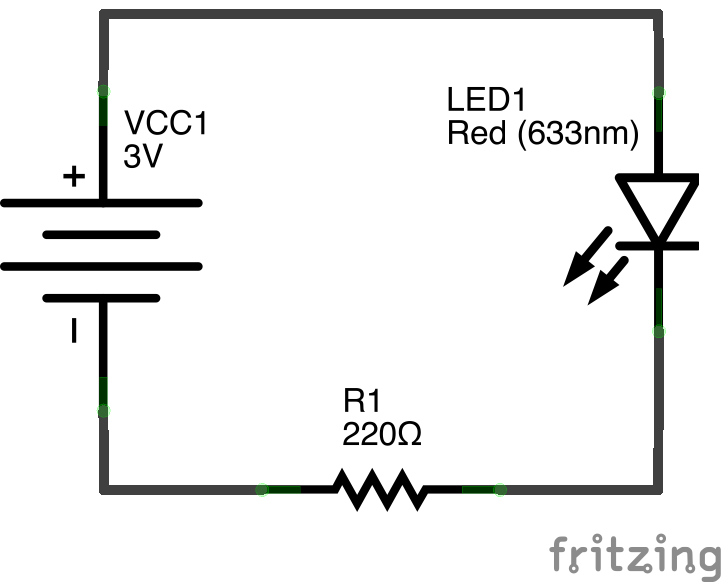
\includegraphics[width=0.3\textwidth]{LED-bateria-diagrama.png} % La imagen esta incluida en el mismo directorio del código
    		\caption{Diagrama eléctrico del circuito a ensamblar.}
    		\label{dia:elecir}
    	\end{center}
    \end{figure}

    Este diagrama eléctrico lo único que nos dice es que tenemos que conectar la parte positiva de nuestra batería a el ánodo de nuestro LED, y el cátodo del LED, a una patita de la resistencia. Después conectamos la otra patita de la resistencia a la parte negativa de la batería y habremos terminado con nuestro circuito eléctrico.

    Pero esto aun no nos da la suficiente información para hacerlo en nuestro protoboard. Esto lo podemos ver en la figura \ref{dia:cir}.

    \begin{figure}[h]
    	\begin{center}
    		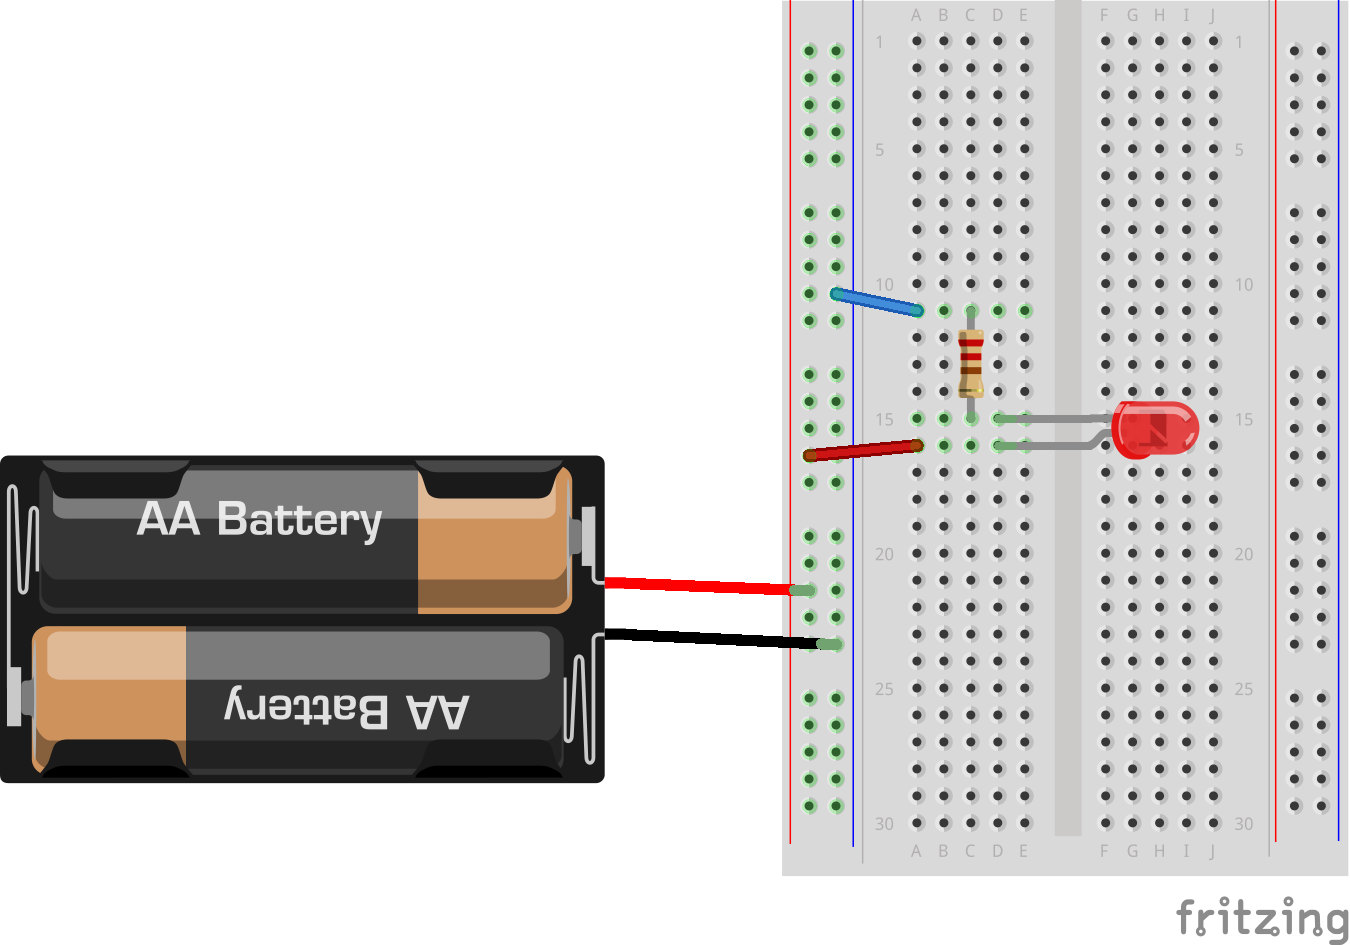
\includegraphics[width=0.5\textwidth]{LED-bateria.png} % La imagen esta incluida en el mismo directorio del código
    		\caption{Diagrama del circuito a ensamblar.}
    		\label{dia:cir}
    	\end{center}
    \end{figure}

    El protoboard tiene conexiones internas, que aprovechamos para hacer nuestro circuito. Primero que nada nuestro protoboard esta dividido en varias partes. La parte central tiene conexiones horizontales, y las secciones laterales tienen conexiones verticales. Una práctica común es conectar el voltaje positivo de alimentación en la columna marcada de rojo en las secciones laterales y el voltaje negativo (o de referencia) en la columna marcada con azul, así siempre tenemos a la mano la alimentación en un circuito complejo (Ver la figura \ref{dia:proto}).

    \begin{figure}[h]
    	\begin{center}
    		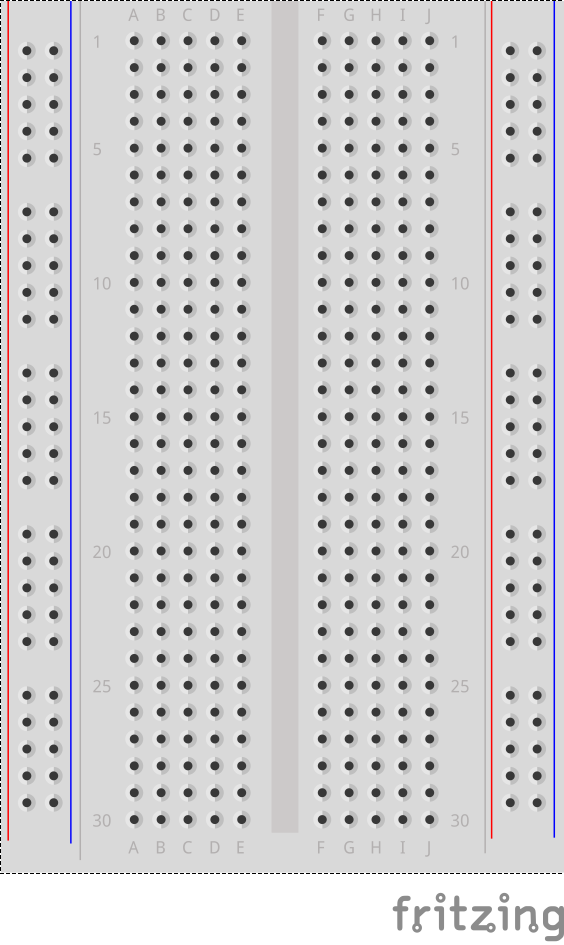
\includegraphics[width=0.25\textwidth]{protoboard.png} % La imagen esta incluida en el mismo directorio del código
    		\caption{Protoboard.}
    		\label{dia:proto}
    	\end{center}
    \end{figure}

    Una vez que tenemos nuestro circuito eléctrico ensamblado, podemos conectarlo a nuestra fuente de alimentación. En caso de que tengas un par de baterías AA con una manera de conectarlas, puedes hacerlo de la manera en que viene indicado en la figura \ref{dia:cir}, pero si no la has conseguido aun, no hay problema. Podemos usar la fuente de alimentación del laboratorio.

    Para usar la fuente de alimentación del laboratorio tenemos que asegurarnos de que este configurada el voltaje que queremos y que la estas conectando de la manera correcta. Por lo que te sugiero que pongas atención en la explicación que se hará en el momento de la práctica.

%----------------------------------------------------------------------------------------
%	CONCLUSIONES
%----------------------------------------------------------------------------------------

\section{Conclusiones}
	El alumno deberá describir sus conclusiones al final de su reporte de práctica.
    
%----------------------------------------------------------------------------------------
%	HOJA DE ANOTACIONES
%----------------------------------------------------------------------------------------

\clearpage
\section{Hoja de Anotaciones}
	Anota los pasos a seguir para utilizar correctamente la fuente de alimentación.

	\begin{enumerate}
		\item
		\item
		\item
		\item 
	\end{enumerate}

	Realiza las mediciones de la resistencia en el primer circuito:

	\begin{center}
		\begin{tabular}{|p{1.5cm}|p{1.5cm}|p{1.5cm}|}
			\hline
			$V$ & $I$ & $R$          \\
			\hline
			    &     & $220 \Omega$ \\
			\hline
			    &     & $330 \Omega$ \\
			\hline
			    &     & $1 k \Omega$ \\
			\hline
		\end{tabular}
	\end{center}

	Realiza las mediciones del LED en el primer circuito:

	\begin{center}
		\begin{tabular}{|p{1.5cm}|p{1.5cm}|p{1.5cm}|}
			\hline
			$V$ & $I$ & $R$ \\
			\hline
			    &     &     \\
			\hline
			    &     &     \\
			\hline
			    &     &     \\
			\hline
		\end{tabular}
	\end{center}

    
%----------------------------------------------------------------------------------------
%	FIN DEL DOCUMENTO
%----------------------------------------------------------------------------------------

\end{document}